%!TEX root = ../thesis.tex
\section{Coffee Berries}

A coffee bean is a seed from the Coffea plant and the source for coffee. This
fruit is often referred to as a coffee cherry, but unlike the cherry, which
usually contains a single pit, it is a berry most commonly found having two
seeds with their flat sides together.

\tagstructbegin{tag=Part}
\begin{figure}[H]
    \centering
    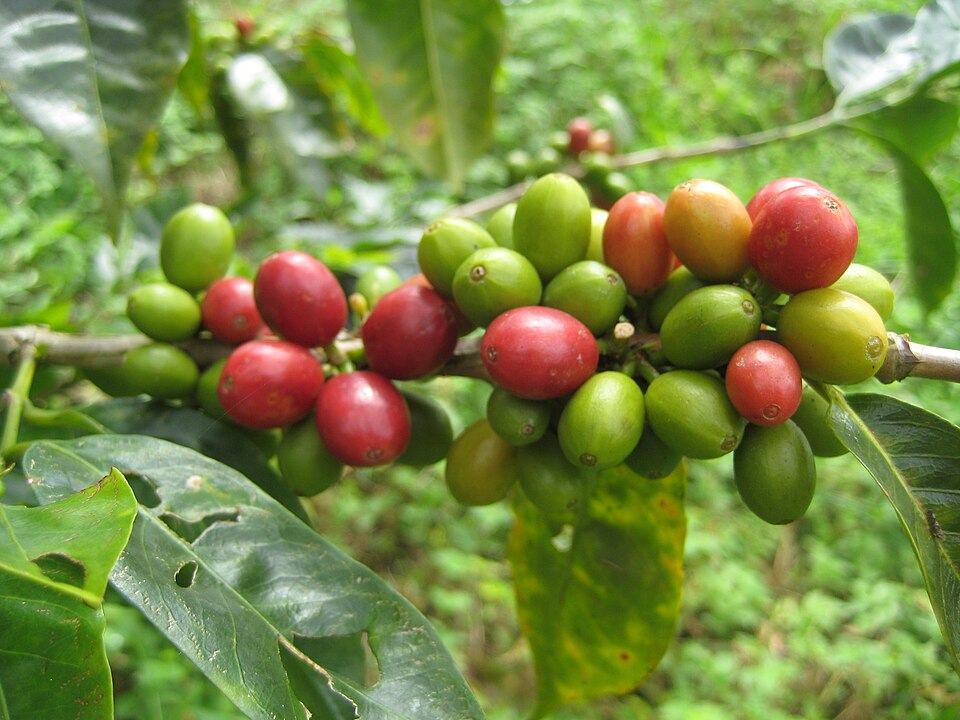
\includegraphics[width=0.6\textwidth,alt={Multiple red and green coffee
    berries clustered together on coffee tree branches}]{
        Clumps_of_coffee_berries_growing_on_a_tree_by_Brian_Smith.jpg
    }
    \caption{Clumps of coffee berries growing on a tree (Photo by Brian Smith)}
    \label{fig:coffee_berries}
\end{figure}
\tagstructend

\subsection{Characteristics of Coffee Berries}

The two most economically important varieties of coffee plants are the arabica
and the robusta; approximately 60\% of the coffee produced worldwide is arabica
and some 40\% is robusta.

\tagstructbegin{tag=Part}
\begin{table}[H]
    \centering
    \caption{Common Coffee Species Comparison}
    \medskip
    \label{tab:coffee_species}
    \renewcommand{\arraystretch}{1.5}
    \tagpdfsetup{table/header-columns={1},table/header-rows={1}}
    \begin{tabular}{|>{\bfseries}l|l|l|}
        \hline
        Species & \textbf{Flavor Profile} & \textbf{Global Production} \\
        \hline
        Arabica & Smooth, complex, with fruit notes & 60\% \\
        \hline
        Robusta & Strong, bitter, earthy & 40\% \\
        \hline
    \end{tabular}
\end{table}
\tagstructend
\pagebreak

The following table summarizes key information about coffee berries:

\tagstructbegin{tag=Part}
\begin{table}[H]
    \centering
    \caption{Key Characteristics of Coffee Berries}
    \medskip
    \label{tab:coffee_characteristics}
    \renewcommand{\arraystretch}{1.5}
    \tagpdfsetup{table/header-columns={1}}
    \begin{tabular}{|>{\bfseries}p{2in}|p{4in}|}
        \hline
        Color at Ripeness & Bright red, yellow or pink depending on variety \\
        \hline
        Size & Approximately 15 mm in diameter \\
        \hline
        Weight & 300--330 mg dry \\
        \hline
        Seeds per Berry & Typically 2 seeds; 10--15\% are peaberries (single seed) \\
        \hline
        Time to Maturity & 6--11 months depending on variety and growing conditions \\
        \hline
        Caffeine Content & 1.0--2.5\% by dry weight \\
        \hline
        Growing Conditions & Altitudes of 600--2,200 meters; temperatures of 15--24°C \\
        \hline
        Shelf Life (Fruit) & 2--3 weeks if left on tree after ripening \\
        \hline
    \end{tabular}
\end{table}
\tagstructend